% !Mode:: "TeX:UTF-8"
%
% 第三章：方法
%
% 本节展示的用法：
%   - 图片插入（figure + includegraphics）
%   - 公式（equation 环境）
%   - 交叉引用（\ref{}）
%

\chapter{方法}
\echapter{Proposed Method}
\label{chap:method}

本章介绍本文提出的方法。图\ref{fig:framework}展示了整体框架。

\begin{figure}[h]
\centering
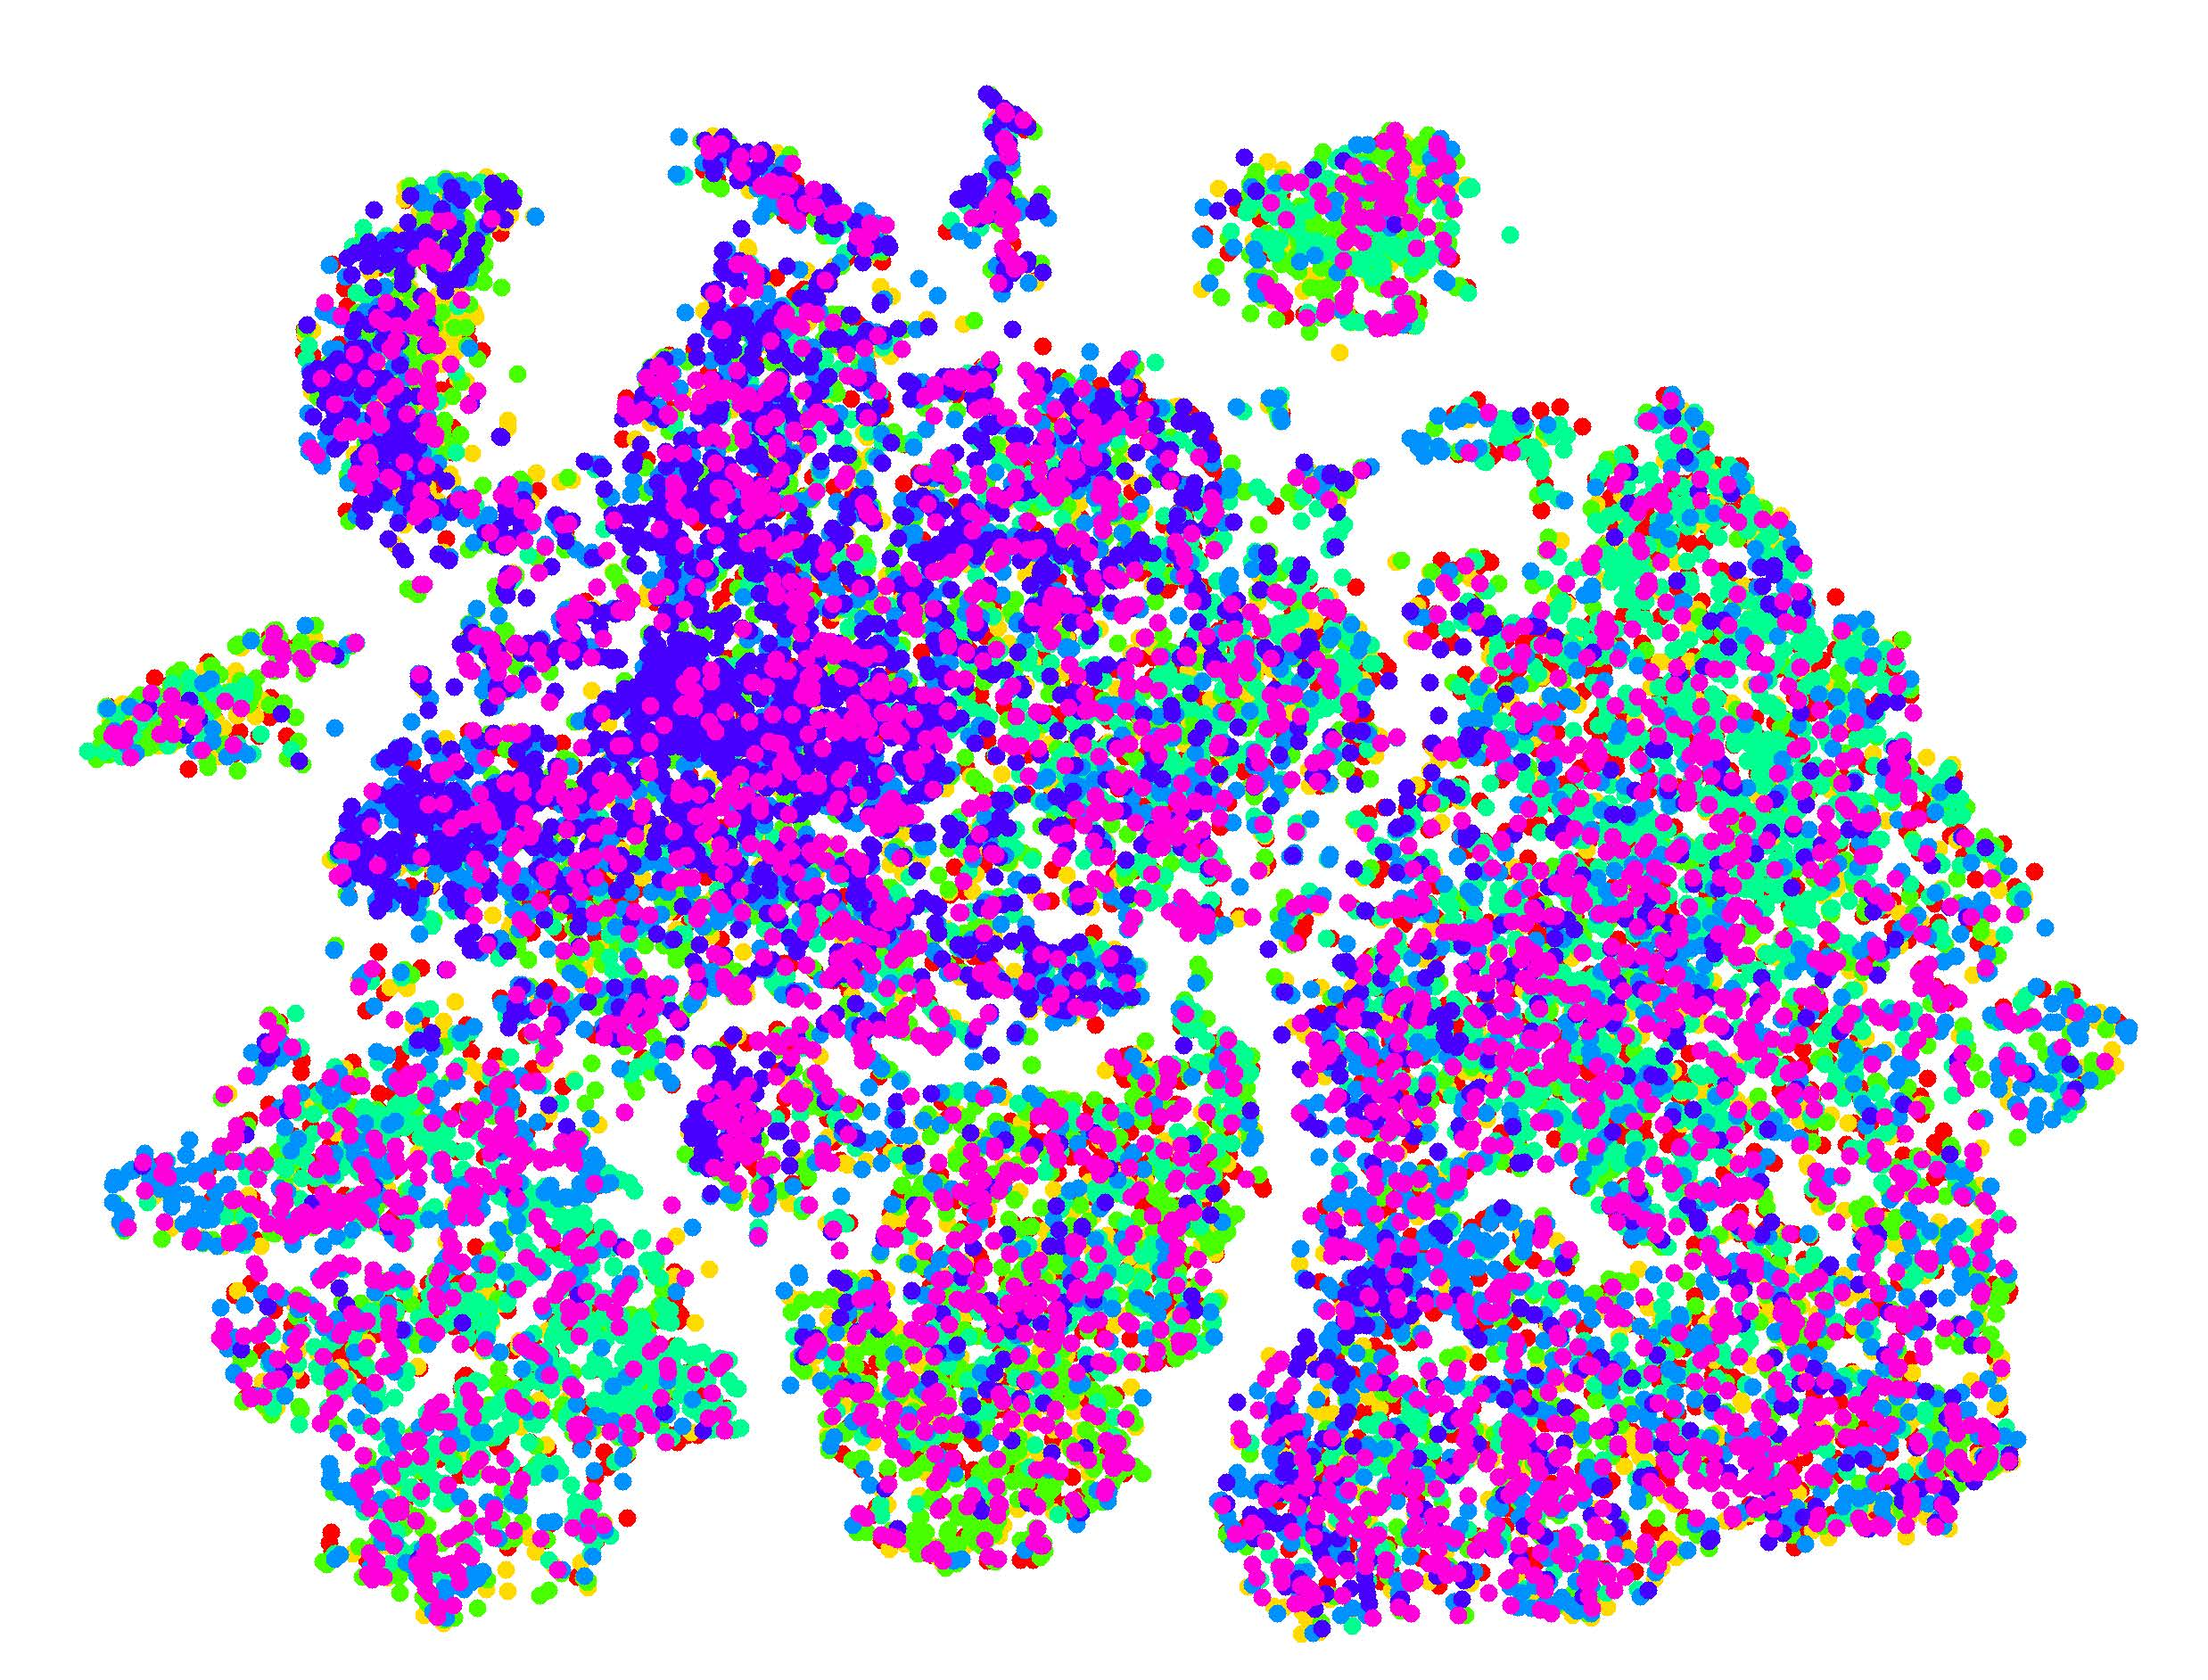
\includegraphics[width=0.6\textwidth]{figures/GIST}
\caption{方法的整体框架示意图}
\label{fig:framework}
\end{figure}

\section{模型定义}
\esection{Model Definition}
\label{sec:model_def}

设输入为 \(x \in \mathbb{R}^d\)，模型输出为
\begin{equation}
\hat{y} = f_\theta(x) = W_2 \cdot \sigma(W_1 x + b_1) + b_2,
\label{eq:model}
\end{equation}
其中 \(\theta = \{W_1, b_1, W_2, b_2\}\) 为可学习参数，\(\sigma(\cdot)\) 为激活函数。

\section{损失函数}
\esection{Loss Function}
\label{sec:loss}

模型通过最小化以下损失进行训练：
\begin{equation}
\mathcal{L}(\theta) = \frac{1}{N} \sum_{i=1}^N \ell(y_i, \hat{y}_i) + \lambda \cdot \Omega(\theta),
\label{eq:loss}
\end{equation}
其中 \(\ell\) 为任务损失（回归用 MSE，分类用交叉熵），\(\Omega\) 为正则项。

\section{训练流程}
\esection{Training Pipeline}

算法\ref{alg:training}总结了完整的训练流程，详见第\ref{chap:implementation}章。

\begin{algorithm}[h]
\caption{训练流程}
\label{alg:training}
\SetAlgoLined
\KwIn{数据集 \(\mathcal{D}\)，初始参数 \(\theta_0\)}
\KwOut{\(\theta^*\)}
\For{epoch = 1 \KwTo \(E\)}{
    \For{每个小批量 \(\mathcal{B} \subset \mathcal{D}\)}{
        \(\theta \leftarrow \theta - \alpha \nabla \mathcal{L}_{\mathcal{B}}(\theta)\)\;
    }
}
\Return \(\theta\)\;
\end{algorithm}
